\documentclass[tikz,border=8pt]{standalone}
\usepackage{amsmath}
\usepackage{lmodern}
\usepackage[T1]{fontenc}
\usetikzlibrary{arrows.meta,calc,decorations.pathreplacing,positioning}

\definecolor{mistyblue}{HTML}{A3BFD9}
\definecolor{slateblue}{HTML}{7A90B2}
\definecolor{sagegreen}{HTML}{A3BFA3}
\definecolor{dustyteal}{HTML}{6E8B8B}
\definecolor{softgray}{HTML}{D8D8D8}
\definecolor{deepmutedblue}{HTML}{4A5A6A}

\begin{document}
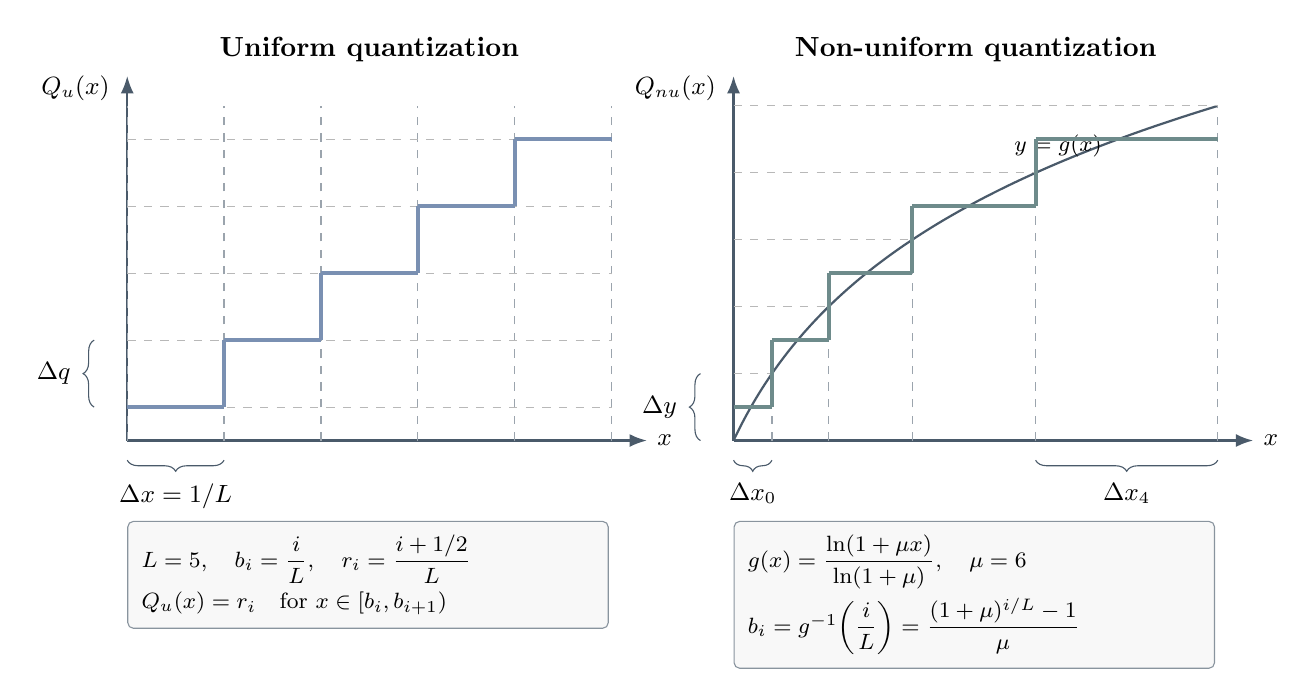
\begin{tikzpicture}[
    >=Latex,
    font=\small,
    axis/.style={deepmutedblue, line width=0.8pt, -{Latex[length=2.2mm]}},
    guide/.style={deepmutedblue!55, dashed, line width=0.45pt},
    level/.style={softgray!85!black, dashed, line width=0.36pt},
    stepu/.style={slateblue, line width=1.45pt},
    stepn/.style={dustyteal, line width=1.45pt},
    curve/.style={deepmutedblue, line width=0.8pt},
    mathbox/.style={draw=deepmutedblue!65, rounded corners=2pt, fill=softgray!18, align=left, inner sep=5pt, font=\footnotesize}
]

% -------- geometry and parameters --------
% L = number of quantization cells, mu = companding factor.
\def\W{6.15}
\def\H{4.25}
\def\L{5}
\def\MU{6}
\def\GAP{1.55}
\pgfmathsetmacro{\Xtwo}{\W+\GAP}

% ================================================================
% LEFT: UNIFORM QUANTIZER
% ================================================================
\node[font=\bfseries\normalsize, text=black] at ({\W/2}, {\H+0.72}) {Uniform quantization};

\draw[axis] (0,0) -- ({\W+0.45},0) node[right, text=black] {$x$};
\draw[axis] (0,0) -- (0,{\H+0.38});
\node[anchor=east, text=black] at (-0.10,{\H+0.22}) {$Q_u(x)$};

% equal input decision boundaries: b_i = i/L
\foreach \i in {0,...,5}{
    \pgfmathsetmacro{\xx}{\W*\i/\L}
    \draw[guide] (\xx,0) -- (\xx,\H);
}
% equal reconstruction levels: r_i = (i+1/2)/L
\foreach \i in {0,...,4}{
    \pgfmathsetmacro{\yy}{\H*(\i+0.5)/\L}
    \draw[level] (0,\yy) -- (\W,\yy);
}
% staircase: discrete output, equal-width bins
\foreach \i in {0,...,4}{
    \pgfmathsetmacro{\xa}{\W*\i/\L}
    \pgfmathsetmacro{\xb}{\W*(\i+1)/\L}
    \pgfmathsetmacro{\ya}{\H*(\i+0.5)/\L}
    \draw[stepu] (\xa,\ya) -- (\xb,\ya);
    \ifnum\i<4
        \pgfmathsetmacro{\yb}{\H*(\i+1.5)/\L}
        \draw[stepu] (\xb,\ya) -- (\xb,\yb);
    \fi
}

% spacing annotations
\draw[decorate, decoration={brace, amplitude=4pt, mirror}, deepmutedblue]
    (0,-0.25) -- ({\W/\L},-0.25)
    node[midway, below=5pt, text=black] {$\Delta x=1/L$};
\draw[decorate, decoration={brace, amplitude=4pt}, deepmutedblue]
    (-0.42,{\H*0.5/\L}) -- (-0.42,{\H*1.5/\L})
    node[midway, left=5pt, text=black] {$\Delta q$};

\node[mathbox, anchor=north west, text=black, text width=5.75cm] at (0,-1.02) {%
$L=5,\quad b_i=\dfrac{i}{L},\quad r_i=\dfrac{i+1/2}{L}$\\[2pt]
$Q_u(x)=r_i\quad \text{for } x\in[b_i,b_{i+1})$};

% ================================================================
% RIGHT: NON-UNIFORM QUANTIZER VIA COMPANDING
% ================================================================
\begin{scope}[xshift=\Xtwo cm]
\node[font=\bfseries\normalsize, text=black] at ({\W/2}, {\H+0.72}) {Non-uniform quantization};

\draw[axis] (0,0) -- ({\W+0.45},0) node[right, text=black] {$x$};
\draw[axis] (0,0) -- (0,{\H+0.38});
\node[anchor=east, text=black] at (-0.10,{\H+0.22}) {$Q_{nu}(x)$};

% Compressor curve used only to compute the non-uniform x boundaries.
\draw[curve, domain=0:1, samples=140, smooth, variable=\t]
    plot ({\W*\t},{\H*ln(1+\MU*\t)/ln(1+\MU)});
\node[anchor=west, text=black, font=\footnotesize] at ({0.56*\W},{0.88*\H}) {$y=g(x)$};

% uniform grid in compressed y, back-projected to x_i = g^{-1}(i/L)
\foreach \i in {0,...,5}{
    \pgfmathsetmacro{\yy}{\H*\i/\L}
    \pgfmathsetmacro{\xx}{\W*(pow(1+\MU,\i/\L)-1)/\MU}
    \draw[level] (0,\yy) -- (\xx,\yy);
    \draw[guide] (\xx,0) -- (\xx,\yy);
}

% staircase: discrete output, unequal-width bins
\foreach \i in {0,...,4}{
    \pgfmathsetmacro{\xa}{\W*(pow(1+\MU,\i/\L)-1)/\MU}
    \pgfmathsetmacro{\xb}{\W*(pow(1+\MU,(\i+1)/\L)-1)/\MU}
    \pgfmathsetmacro{\ya}{\H*(\i+0.5)/\L}
    \draw[stepn] (\xa,\ya) -- (\xb,\ya);
    \ifnum\i<4
        \pgfmathsetmacro{\yb}{\H*(\i+1.5)/\L}
        \draw[stepn] (\xb,\ya) -- (\xb,\yb);
    \fi
}

% compare two input cell widths
\pgfmathsetmacro{\xzero}{\W*(pow(1+\MU,0/\L)-1)/\MU}
\pgfmathsetmacro{\xone}{\W*(pow(1+\MU,1/\L)-1)/\MU}
\pgfmathsetmacro{\xfour}{\W*(pow(1+\MU,4/\L)-1)/\MU}
\pgfmathsetmacro{\xfive}{\W*(pow(1+\MU,5/\L)-1)/\MU}
\draw[decorate, decoration={brace, amplitude=4pt, mirror}, deepmutedblue]
    (\xzero,-0.25) -- (\xone,-0.25)
    node[midway, below=5pt, text=black] {$\Delta x_0$};
\draw[decorate, decoration={brace, amplitude=4pt, mirror}, deepmutedblue]
    (\xfour,-0.25) -- (\xfive,-0.25)
    node[midway, below=5pt, text=black] {$\Delta x_4$};
\draw[decorate, decoration={brace, amplitude=4pt}, deepmutedblue]
    (-0.42,0) -- (-0.42,{\H/\L})
    node[midway, left=5pt, text=black] {$\Delta y$};

\node[mathbox, anchor=north west, text=black, text width=5.75cm] at (0,-1.02) {%
$g(x)=\dfrac{\ln(1+\mu x)}{\ln(1+\mu)},\quad \mu=6$\\[2pt]
$b_i=g^{-1}\!\left(\dfrac{i}{L}\right)=\dfrac{(1+\mu)^{i/L}-1}{\mu}$};
\end{scope}

\end{tikzpicture}
\end{document}
